\section{Preliminaries}

\subsection{Notation}
The set of integers and real numbers are denoted $\int$ and $\real$ respectively. A ranged subset of a space is denoted with $\mathbb{S}\rii{i}{j}=\{s\in\mathbb{S}|i\leq s\leq j\}$. Open bounds are defined using notation such as $\mathbb{S}\rgeq{i}$. Define the set of integers from $1$ to $k>1$ as $\idxset{k}\triangleq\int\rii{1}{k}$.

A directed graph with $\gnumnodes\in\int\rgeq{1}$ nodes is defined as $\graph\triangleq\{(\gnodeedges{n},\gnodelabel{n})\}_{n\in\idxset{\gnumnodes}}$ where $\gnodeedges{n}\subseteq\idxset{\gnumnodes}$ lists the successor nodes of node $n$ and $\gnodelabel{n}\in\idxset{\gnumlabels}$ is an integer label assigned to node $n$ where $\gnumlabels$ is the max integer label. A discrete, time varying function, $f:\int\rgeq{0}\rightarrow\idxset{\gnumnodes}$, is said to respect the graph if $f(t)=n$ implies that $f(t+1)\in\gnodeedges{n}$. The set of all such functions for a specific graph, $\graph$ is denoted $\Sigma(\mathcal{G})\triangleq\{g:\int\rgeq{0}\rightarrow\idxset{\gnumnodes}\ |\ g(\cdot)\text{ respects }\graph\}$. 
\begin{remark}
Note that a function $f(\cdot)\in\Sigma(\graph)$ maps to a node, not the node's label. The active label at time $t$ can be accessed with $\gnodelabel{f(t)}$. 
\end{remark}

\subsection{Switching Signals}
An external switching signal is a discrete function, $\ss:\int\rgeq{0}\rightarrow \idxset{\gnumnodes}$, that is uninfluenced by the system's state and control inputs and causes elements of the plant and/or controller to switch. In this work, the switching signals are constrained using directed graphs such that, given the graph $\graph$, $\ss(\cdot)\in\Sigma(\graph)$. At time $t$, the active node's label indicates the system's mode and is defined as $\ssl(t)\triangleq \gnodelabel{\ss(t)}$. Using directed graphs to constrain the switching signal generalizes dwell time and successor constraints from previous literature such as \cite{Danielson2019, Hall2022, Zhang2016}, representing a richer set of constraints, as shown in \autoref{fig:graph_ex}.

\begin{figure}[t]
\centering
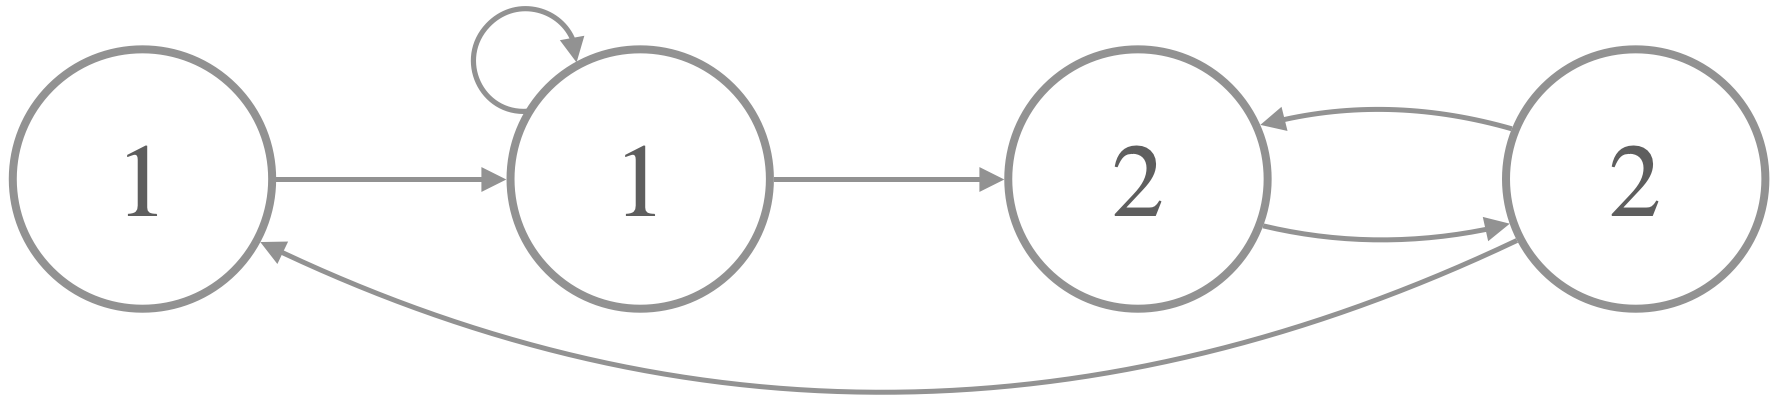
\includegraphics[scale=0.15]{./figures/graph_remark}
\caption{A graph representing a 2-mode system. The system is in mode 1 when node 1 or 2 is active and in mode 2 otherwise. Note that, when the system switches to mode 1 by entering node 1, it must ``dwell'' in mode 1 for at least 2 steps. This is equivalent to a minimum dwell time constraint found in works such as \cite{Danielson2019}.}
\label{fig:graph_ex}
\end{figure}

Prior knowledge of the switching signal is not required, but its value at time $t$ is known immediately. Furthermore, its directed graph is known at design time. 
\subsection{General Constrained Switched Systems}
Switched systems, in the context of this work, are comprised of \nummodes modes and a graph based switching constraint, $\graph$, where the labels of the graph correspond to the system's mode indices, $\nummodes=\gnumlabels$. Each mode contains the dynamics and constraints that the system must respect while the mode is active. The mode corresponding to index \modeidx is denoted by the tuple
\begin{equation}
\mode{\modeidx}\triangleq\{f_\modeidx\in \mathcal{D}^{\nx,\nu,\nw}, \xcon[\modeidx]\subseteq\real^\nx, \ucon[\modeidx]\subseteq\real^\nu, \wcon[\modeidx]\subset\real^\nw\}\nonumber
\end{equation}
where $\mathcal{D}^{\nx,\nu,\nw}\triangleq\{f:\real^{\nx\times\nu\times\nw}\rightarrow\real^\nx\}$ defines the set of discrete dynamics,  and $\xcon[\modeidx]$, $\ucon[\modeidx]$, and  $\wcon[\modeidx]$ are the state, input, and disturbance constraints respectively. The full constrained switched system collects the modes and directed graph into
\begin{equation}\label{eq:basic_switched_sys}
\modes\triangleq\{\{\mode{\modeidx}\}_{\modeidx\in\idxset{\nummodes}}, \graph\}.
\end{equation}

\subsection{Set Operations and Control Invariance}
Set operations provide tools to analyze how a mode evolves under allowable inputs. Given a mode, $\mode{\modeidx}$, the following important set operation is introduced. 
\begin{definition}[Previewed Robust Preset]\label{def:prev_robust_preset}
The $k$-step, previewed robust preset of a set $\mathcal{S}$ under the constrained dynamics $\mode{\modeidx}$ is given by
\begin{align}
\PreviewedPre[\modeidx][0]{\mathcal{S}}&\triangleq\mathcal{S},\\
\PreviewedPre[\modeidx][k]{\mathcal{S}}&\triangleq\{x\in\xcon[\modeidx]|\forall w\in\wcon[\modeidx],\exists u\in\ucon[\modeidx]\text{ s.t. }\nonumber\\
&\hspace{1.85cm} f_\modeidx(x,u,w)\in\PreviewedPre[\modeidx][k-1]{\mathcal{S}}\}.
\end{align}
\end{definition}
Comparing this to the more common robust preset operator, the previewed robust preset is allowed to select the input based on a known disturbance. The previewed robust preset is used when the system is allowed a preview of the current disturbance. This preview can expand the size of the preset because the selected input need not handle every possible disturbance. 

For linear systems where $f_\modeidx(x,u,w) = A_\modeidx x + B_\modeidx u + E_\modeidx w$, previewed robust presets can be found using basic set operations such as the Minkowski sum and difference as shown below and adapted from \cite{Borrelli2017}.
\begin{align*}
\PreviewedPre[\modeidx][1]{\mathcal{S}} &= \left(\left(\left(\mathcal{S}\oplus\left(-B_\modeidx\circ\ucon[\modeidx]\right)\right)\ominus E_\modeidx\circ\wcon[\modeidx]\right)\circ A_\modeidx\right)\ \cap\ \xcon[\modeidx].
\end{align*}

Preset operations are critical in the calculation of invariant sets commonly used in feasibility analysis. Control invariant and previewed-robust control invariant sets are defined as follows.
\begin{definition}[\Ac{ci} sets \cite{Dorea1999}]\label{def:ci_set}
A set, $\mathcal{S}\subseteq\xcon[\modeidx]$ is CI under mode $\mode{\modeidx}$ if for all $x\in\mathcal{S}$, there exists a $u\in\ucon[\modeidx]$ such that $f_\modeidx(x,u,0)\in\mathcal{S}$. Likewise, a set $\mathcal{S}\subseteq\xcon[\modeidx]$ is a previewed robust CI (PR-CI) set if, for all $x\in\mathcal{S}$ and $w\in\mathcal{W}_\modeidx$, there exists a $u\in\ucon[\modeidx]$ such that $f_\modeidx(x,u,w)\in\mathcal{S}$. Equivalently, $\mathcal{S}$ is CI (PR-CI) iff $\mathcal{S}\subseteq\Pre[\modeidx][1]{\mathcal{S}}$ where the preset operator is nominal (previewed robust).
\end{definition}

A final tool used in this paper is the convex hull of a set defined as follows.
\begin{definition}[Convex Hull]
Given a set $\mathcal{S}\subseteq\real^n$, the convex hull is defined as 
\begin{align*}
&\Call{ConHull}{\mathcal{S}}\triangleq\\&\{x\in\real^n\ |\ \exists\ a,b\in\mathcal{S},\ \gamma\in\real\rii{0}{1}\ \text{s.t.}\ x=\gamma a + (1-\gamma)b\}.
\end{align*}
\end{definition}
\subsection{Feasibility Analysis}
In the introduction, it was mentioned that constraining the external switching signal allows a time-invariant feasible region to be replaced with a time-varying one. This work describes these time-varying feasible regions using safe-set collections. These are collections of sets, indexed by the switching signal, that serve as time-varying state constraints of the system. To establish persistent feasibility, every safe-set must be within the 1-step preset of all possible successor safe-sets. This is presented formally in the following definition.
\begin{definition}[Safe-set collection]
Let the external switching signal, $\ss\in\Sigma(\graph)$ govern the system $\modes\triangleq\{\{\mode{\modeidx}\}_{\modeidx\in\idxset{\nummodes}}, \graph\}$. A collection of sets indexed by the nodes of $\graph$, $\mathcal{S}=\{\mathcal{S}_{i}\}_{i\in\idxset{\gnumnodes}}$ is a safe-set collection if
$$\mathcal{S}_{i}\subseteq\Pre[\gnodelabel{j}][1]{\mathcal{S}_{j}}\ \forall\ i\in\idxset{\gnumnodes},\ j\in \gnodeedges{i}$$
\end{definition}
Safe set collections create target sets for the system to move into at each time step. The preset condition ensures that, no matter how $\ss$ evolves, there will always be a feasible input that moves the state into the current target set.
